\chapter{Discussion}
\label{chp:discussion}
\todo[inline]{Mer diskusjon?}
In this project, a mathematical method was developed. Not much empirical analysis was done to estimate the performance of the method, so the amount of further discussion is somewhat limited, but there are some things to be said about when the method will be valid, and how precise it will be. 

\begin{figure}
 \centering
 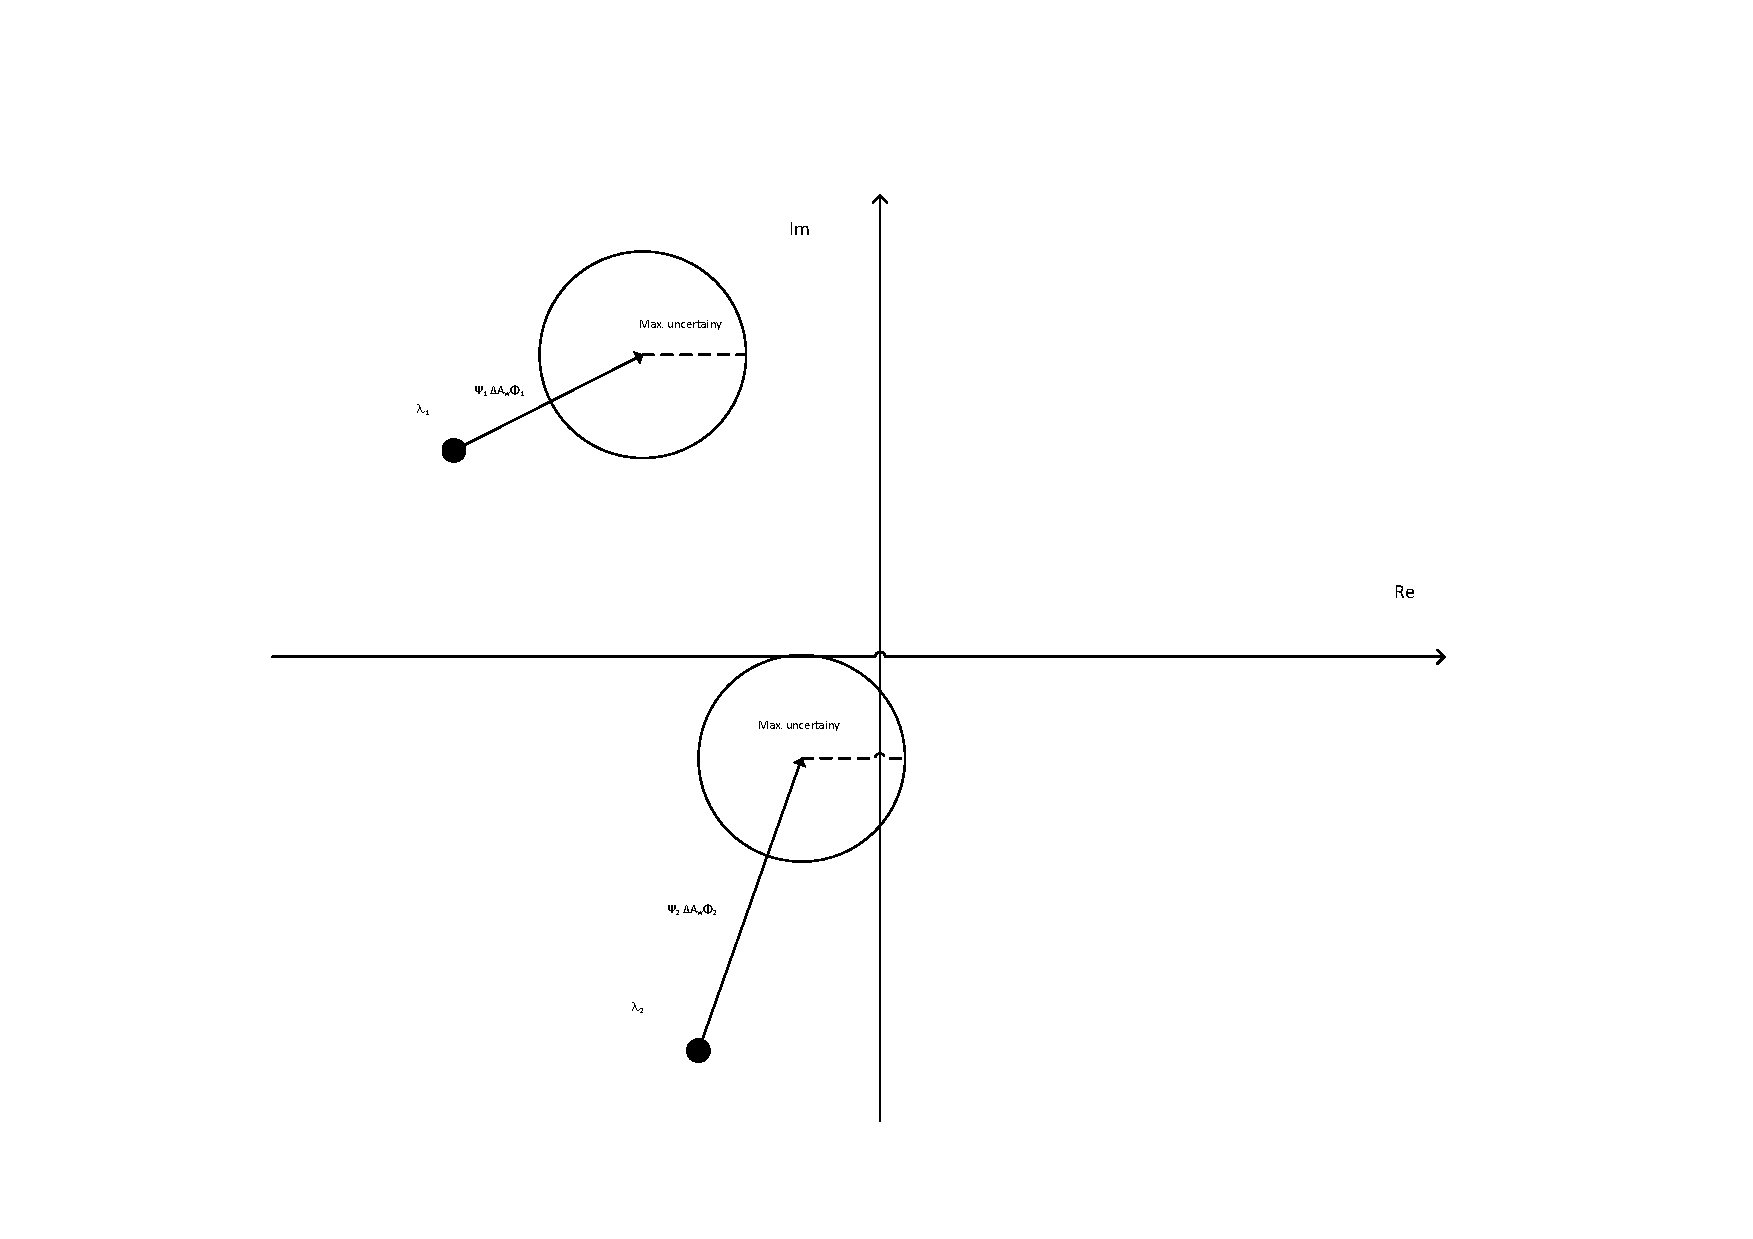
\includegraphics[width=\textwidth,height=\textheight,keepaspectratio]{Figures/Pole_changes.pdf}
 \caption{The estimate of $\lambda_1$ is somewhat stable, while there is a certain risk for $\lambda_2$ to become unstable}
 \label{fig:figure_of_the_method}
\end{figure}{}


\section{Guarantees of the estimate}
\label{sec:guarantees_of_estimate}
The difference between a real exponential and a Taylor-estimate is very dependant on if the exponent is larger than 0 or not. Just as a simple example, the two figures \cref{fig:fast_taylor} and \cref{fig:slow_taylor} shows how the difference between a Taylor-estimate and the real series develops with the number of steps in the Taylor-approximation. The sampling-rate should usually be fast enough to not be affected by the fastest dynamics, but it does not need to be true for stable dynamics. In practice, this might result in an algorithm that will give poor upper bounds for stiff systems. Since a circuit may contain very fast capacitors or indicators, a factor $e^{\norm{\Vec{A_s} T_s}}$ that becomes $e^100$ might be unlikely, but not that unreasonable. As seen from the graph, the result of such a matrix is that roughly 60 terms are needed to get rid of the most dramatic uncertainties. 
\begin{figure}
 \centering
 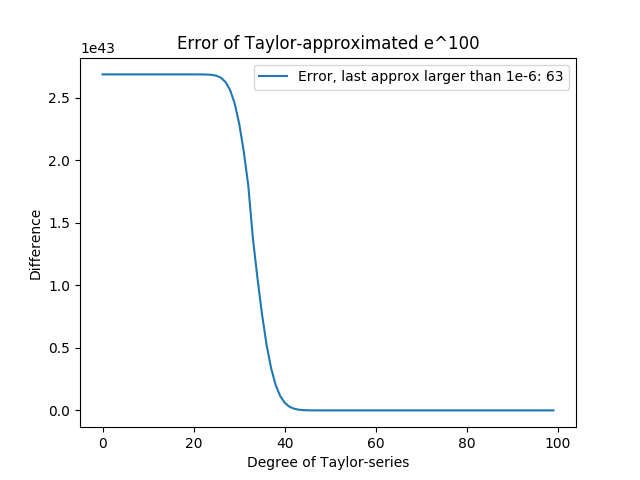
\includegraphics[width=\textwidth,height=\textheight,keepaspectratio]{Figures/taylor_estimate.png}
 \caption{Difference between real value and Taylor-estimate for $e^100$}
 \label{fig:fast_taylor}
\end{figure}{}

\begin{figure}
 \centering
 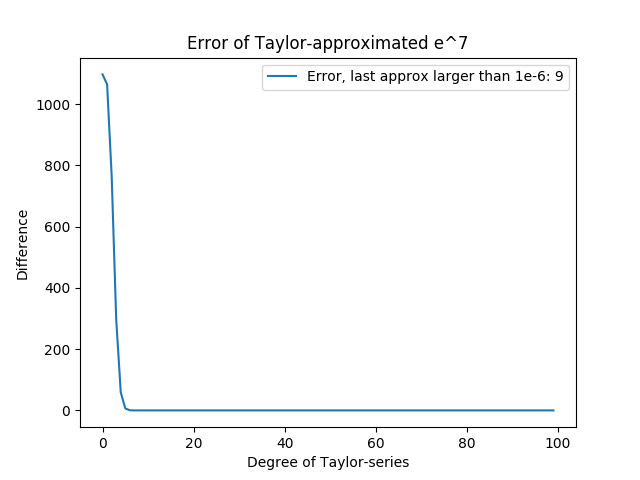
\includegraphics[width=\textwidth,height=\textheight,keepaspectratio]{Figures/taylor_estimate_slow_dyynamics.png}
 \caption{Difference between real value and Taylor-estimate for $e^3$}
 \label{fig:slow_taylor}
\end{figure}{}

\noindent
The true value of the estimates given by figures like \cref{fig:fast_taylor} and \cref{fig:slow_taylor} is that both the norm of $\Vec{A_s}$ and the norm of the derivative can be calculated before any more expensive computations are made. As can be seen from the plots, the Taylor-series has a certain number of steps that has to be exceeded before the precision starts increasing quickly. As a result, it is possible to say something about the number of steps in the Taylor-series that are needed to get a decent estimate. It even makes it possible to tell if the analysis will be worth it before any expensive computations have to be made. 

\section{Properties of electrical grids}

In the project, a lot of work had to be done in order to handle eigenvalues that are equal to zero. All RLC-circuits are passive systems, which in the case of linear systems also means that they are stable. As a result, there are cases where it might be reasonable to assume that no eigenvalues are equal to 0. Even when the system is not passive. There are still some issues with almost singular systems. The inverse of a system that is almost singular has always at least one eigenvalue that goes towards infinity. As a result, the norm of such a system will be very large and may be difficult to handle, since it will affect the norm of the inverted matrix quite severely. Depending on how quickly Taylor-series tend towards 0, the problem with ill-conditioned matrices might be a large one, or not bad at all. More testing with Taylor-series is most likely required. 
\noindent
The methods developed are also highly dependant on the type of problem that it is used on. In this project, it was assumed that it was very important that the system would not become unstable. Even more so than what is usually required in stability-analysis. This was done at the cost of scalability and ease of use. It is quite possible that, if other properties, like the non-linearities of a problem play a larger role than the time-delay, other methods will be much more useful. Finally, since all controller-parameters are described directly in the z-domain, it is much easier to analyze their effects on the w-domain. 


